\documentclass[12pt]{article}
\usepackage{fullpage}
\usepackage{nopageno}
\usepackage{ifthen}
\usepackage{amsmath}
\usepackage{amssymb}
\usepackage{graphicx} 
\usepackage{version}
\usepackage{amsthm}
%\usepackage{add-copyright}

\excludeversion{solution}

\DeclareMathOperator{\ft}{ft}

\newcommand{\R}{\mathbb{R}}

\title{Take-Home Quiz 5}
\author{Math 131 Section 22}
\date{Due Monday, November 14, 2005}

\newcounter{problem}
\setcounter{problem}{1}

\newenvironment{problem}[1][]
{\begin{flushleft}\hangindent=1em\hangafter=1\noindent\textbf{Problem \arabic{problem}.}
\ifthenelse{\equal{#1}{}}{}{
\textbf{(#1 \ifthenelse{\equal{#1}{1}}{point}{points}).}}
}
{\addtocounter{problem}{1}\end{flushleft}}

\begin{document}
\maketitle

The word problems on this quiz are classics---problems which everyone
who does calculus ought to see.  I hope you will enjoy them.

\begin{problem}[2]
I give you an empty tank of water\footnote{I also give you an empty
box filled with gold.}; the tank is cylindrical, with a radius of $10
\ft$ and a height of $3 \ft$.  I am pouring water into your tank at a
rate of $50\pi \ft^3/\sec$.  How fast is the water level rising?
\end{problem}

\begin{solution}
\subsection*{Solution}

Consider only the water---the height of the tank was given only as an
amusing detail.  Let $V(t)$ be the volume of the water at time $t$,
and $h(t)$ be the height of the water at time $t$.  Since a cylinder
of radius $r = 10$ and height $h$ has volume $\pi r^2 h = 100 \pi h$, we conclude that
$$
V(t) = 100 \pi \cdot h(t).
$$
Differentiating both sides with respect to $t$ gives a relationship
between the rate of volume change and the rate of height change, namely,
$$
\frac{dV}{dt} = 100 \pi \frac{dh}{dt}.
$$
Thus if I am pouring water into the tank at a rate of
$\frac{dV}{dt} = 50\pi \ft^3/\sec$, we solve to find that
$$
\frac{dh}{dt} = 1/2 \ft/\sec,
$$
so the water is increasing in height at a rate of $0.5$ feet per
second.
\end{solution}

%\pagebreak

\noindent
\parbox[b]{3in}{\begin{problem}[2] Everything is dark.  Thankfully,
there is an $8 \ft$ tall lamp behind you.  You are $5 \ft$ tall, and
you are walking away from that lamp at a speed of $3 \ft/\sec$. How
fast is your shadow growing in length?
\end{problem}}
\raisebox{-0.8in}{\parbox[t]{3in}{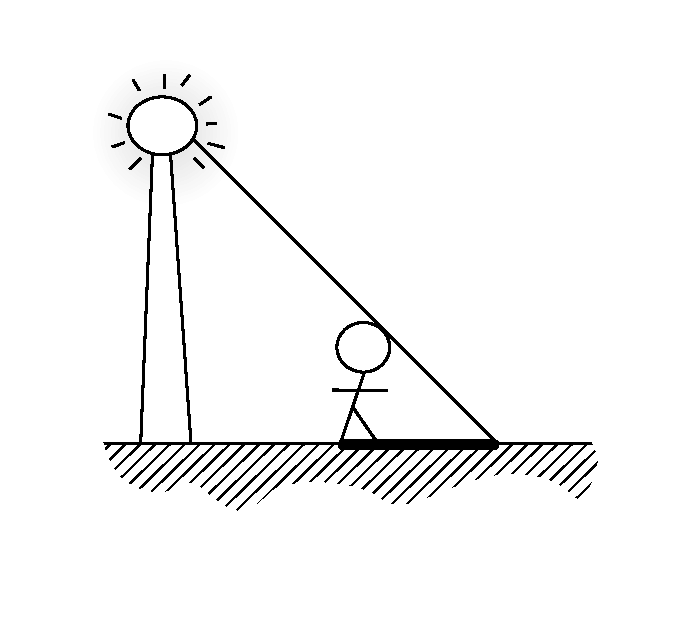
\includegraphics[width=3in]{shadow.ps}}}

\begin{solution}
\subsection*{Solution}
Let $s(t)$ be the length of the shadow at time $t$, and $x(t)$ be the
distance between your feet and the bottom of the lamp's post at time
$t$.  Then by similar triangles\footnote{If you aren't familiar with
how this argument goes, please ask!}, we know
$$
\frac{x(t) + s(t)}{s(t)} = \frac{8}{5},
$$
so rearranging, we get that $5 \cdot x(t) + 5 \cdot s(t) = 8 s(t)$, and solving, we get $3 \cdot s(t) = 5 \cdot x(t)$.  Differentiating both sides with respect to $t$ gives
$$
3 \frac{ds}{dt} = 5 \frac{dx}{dt}.
$$
But $dx/dt$ is the speed with which you are walking, which is $3 \ft/\sec$, so
$$
3 \frac{ds}{dt} = 5 \cdot 3 \ft/\sec,
$$
and thus $ds/dt = 5 \ft/\sec$, which is how fast the shadowing is
growing.
\end{solution}

% \pagebreak

\parbox[b]{3in}{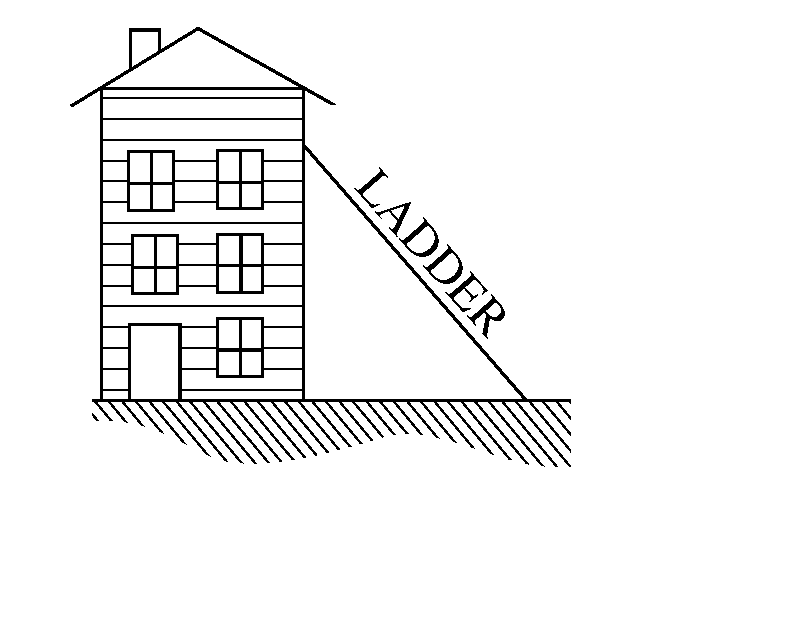
\includegraphics[width=3in]{ladder-sliding-down-house.ps}}
\raisebox{0.3in}{\parbox[b]{3in}{\begin{problem}[3] I have placed my ladder against the
side of my house.  As I pull the bottom of my ladder away from my
house, the top of the ladder slides down the house, as shown.  The
ladder is $25 \ft$ long, and the bottom of my ladder is currently $15
\ft$ from my house.  I am pulling the bottom of the ladder at a speed
of $1 \ft/\sec$.  How fast is the top of the ladder falling?
\end{problem}}}

\begin{solution}
\subsection*{Solution}

Let $x(t)$ be the distance between the base of the ladder and the side
of my house, and $y(t)$ be the distance between the top of the ladder
and the bottom of my house.  Since my home is not yet falling over,
the side of my house makes a right angle to the ground, and so by the
Pythagorean theorem, I deduce that $x(t)^2 + y(t)^2 = 25^2$.

Differentiating with respect to $t$ gives
$$
2 \cdot x(t) \cdot x'(t) + 2 \cdot y(t) \cdot y'(t) = 0.
$$
which relates the current location of the ladder and the rate at
which the ladder is moving.  At some time $t$, I am told that $x(t) =
15 \ft$, and so by the Pythagorean theorem, $y(t) = 20 \ft$.  Also $x'(t) = 1 \ft/\sec$ because I am pulling the bottom of the ladder away at that speed.  Plugging in gives
$$
2 \cdot 15 \cdot 1 + 2 \cdot 20 \cdot y'(t) = 0,
$$ 
so solving for $y'(t)$ gives $y'(t) = -3/4$, and thus the top of
the ladder is falling at a rate of $3/4$ feet per second as I pull the
bottom of the ladder away.

\end{solution}

% \pagebreak

\begin{problem}[1]
I keep pulling the ladder in the previous problem.  The bottom of the
ladder is now $24.99999 \ft$ away from the side of my house, and I am
still pulling the bottom of the ladder away from my house at a speed
of $1 \ft/\sec$.  What sound do I hear?
\end{problem}

\begin{solution}
\subsection*{Solution}

In the previous problem, we discovered that
\begin{equation}
2 \cdot x(t) \cdot x'(t) + 2 \cdot y(t) \cdot y'(t) = 0
\label{relation}
\end{equation}
Now $x(t) = 24.99999\ft$, but $x'(t)$ is still $1 \ft/\sec$.  To find $y(t)$, we use the Pythagorean theorem to calculate
$$
y(t) = \sqrt{25^2 - x(t)} = \sqrt{25^2 - 24.99999^2}.
$$
Plugging in to equation~(\ref{relation}), we get that
$$
y'(t) = \frac{- 2 \cdot 24.99999 \cdot 1}{2 \sqrt{25^2 - 24.99999^2}} \approx -1118 \ft/sec.
$$
But the speed of sound at sea level is $1116 \ft/\sec$, so the tip
of my ladder will be going faster than the speed of sound, and I will
hear a sonic boom!

Of course, a much more likely conclusion is that something has gone
wrong with the mathematical model, and indeed, claiming that falling
ladders are a good way to break the sound barrier is a good way to be
disappointed.
\end{solution}

% \pagebreak

\begin{problem}[2]
Assume that the following equation defines a differentiable function
of $x$.  Calculate $dy/dx$ using implicit differentiation:
$$
x^2 y = 1 + y^2 x.
$$
\end{problem}

\begin{solution}
\subsection*{Solution}
We calculate
\begin{eqnarray*}
\frac{d}{dx} \left( x^2 y \right) &=& \frac{d}{dx} \left( 1 + y^2 x \right) \\
\frac{d}{dx} \left( x^2 \right) y + x^2 \frac{dy}{dx} &=& 
\frac{d}{dx} \left( y^2 \right) x + y^2 \frac{d}{dx} \left( x \right) \\
2xy + x^2 \frac{dy}{dx} &=& 2 x y \frac{dy}{dx} + y^2 \cdot 1 \\
\end{eqnarray*}
So we rearrange to get
$$
\left( x^2 - 2xy \right) \frac{dy}{dx} = y^2 - 2xy 
$$
and therefore, assuming $x^2 - 2xy$ is nonzero, we conclude
$$
\frac{dy}{dx} = \frac{y^2 - 2xy}{x^2 - 2xy}.
$$
\end{solution}

% \pagebreak

\begin{problem}[2]
Assume that the following equation defines a differentiable function
of $x$.  Calculate the slope of the tangent line at a point $(x,y)$ satisfying
$$
x^3 + xy^2 = 2y^2.
$$
\end{problem}

\begin{solution}
\subsection*{Solution}
The slope of the tangent line is just the derivative, so we differentiate:
\begin{eqnarray*}
\frac{d}{dx} \left( x^3 + xy^2 \right) = \frac{d}{dx} \left( 2y^2 \right) \\ 
3x^2 + \frac{d}{dx} \left( xy^2 \right) = 2 \frac{d}{dx} \left( y^2 \right) \\ 
3x^2 + y^2 + x \frac{d}{dx} \left( y^2 \right) = 4 y \frac{dy}{dx} \\
3x^2 + y^2 + 2xy \frac{dy}{dx} = 4 y \frac{dy}{dx}, \\
\end{eqnarray*}
and consequently,
$$
3x^2 + y^2 = (4y - 2xy) \frac{dy}{dx}, \\
$$
so if $4y - 2xy \neq 0$, we conclude,
$$
\frac{dy}{dx} = \frac{x^2 + y^2}{4y - 2xy}.
$$
Note that since $(0,0)$ is on the graph of $x^3 + xy^2 = 2y^2$,
there do exist points where $4y - 2xy$ is zero, so the above
calculation will sometimes fail!  We shouldn't be too
disappointed---it can be hard to see when the solution to an implicit
equation is differentiable!
\end{solution}




\end{document}
